\begin{enumerate}[label=\thechapter.\arabic*,ref=\thechapter.\theenumi]
\item Consider the signals $x\brak{n}$=$2^{n-1} u\brak{ -n+2}$ and $y\brak{n}$=$2^{-n+2}u\brak{ n+1}$, where $u\brak{n}$ is the unit step sequence. Let $X\brak{e^{j\omega}}$ and $Y\brak{e^{j\omega}}$ be the discrete-time Fourier of $x\brak{n}$ and $y\brak{n}$,respectively. The value of the integral $\frac{1}{2\pi}\int_{0}^{2\pi} X\brak{e^{j\omega}} Y\brak{e^{-j\omega}} d \omega$
(rounded off to one decimal place) is \underline{{\hspace{1.5in}}}\\
\hfill{(GATE EC 41 2021)}\\
\solution
\documentclass[journal,12pt,twocolumn]{IEEEtran}
\usepackage{cite}
\usepackage{amsmath,amssymb,amsfonts,amsthm}
\usepackage{algorithmic}
\usepackage{graphicx}
\usepackage{textcomp}
\usepackage{xcolor}
\usepackage{listings}
\usepackage{enumitem}
\usepackage{mathtools}
\usepackage{gensymb}
\usepackage{comment}
\usepackage[breaklinks=true]{hyperref}
\usepackage{tkz-euclide}
\usepackage{gvv} 
\def\inputGnumericTable{} 
\usepackage[latin1]{inputenc} 
\usepackage{color} 

\newtheorem{theorem}{Theorem}[section]
\newtheorem{problem}{Problem}
\newtheorem{proposition}{Proposition}[section]
\newtheorem{lemma}{Lemma}[section]
\newtheorem{corollary}[theorem]{Corollary}
\newtheorem{example}{Example}[section]
\newtheorem{definition}[problem]{Definition}
\newcommand{\BEQA}{\begin{eqnarray}}
\newcommand{\EEQA}{\end{eqnarray}}
\newcommand{\define}{\stackrel{\triangle}{=}}
\theoremstyle{remark}
\newtheorem{rem}{Remark}

\begin{document}

\bibliographystyle{IEEEtran}
\vspace{3cm}

\title{GATE 2022-IN}
\author{EE23BTECH1205 - Avani Chouhan$^{*}$}
\maketitle
\newpage
\bigskip

\renewcommand{\thefigure}{\theenumi}
\renewcommand{\thetable}{\theenumi}

\vspace{3cm}
\textbf{Question : 18} \\
A signal \( x(t) \) is band-limited between 100 Hz and 200 Hz. A signal \( y(t) \) is related to \( x(t) \) as follows:\\

\( y(t) = x(2t - 5) \)\\
The statement that is always true is \\

\begin{enumerate}
  \item[(A)] \( y(t) \) is band-limited between 50 Hz and 100 Hz
  \item[(B)] \( y(t) \) is band-limited between 100 Hz and 200 Hz
  \item[(C)] \( y(t) \) is band-limited between 200 Hz and 400 Hz
  \item[(D)] \( y(t) \) is not band-limited 
\end{enumerate}

\hfill{(GATE IN 2022)}\\
\textbf{Solution:} \\
\begin{align}
x(t) &\rightleftharpoons X(\omega) \label{eq1}\\
x(at) &\rightleftharpoons \frac{1}{|a|} X\left(\frac{\omega}{a}\right) \label{eq2}\\
x(2t) &\rightleftharpoons \frac{1}{2} X\left(\frac{\omega}{2}\right) \label{eq3}\\
x(t - t_0) &\rightleftharpoons e^{-j\omega t_0}X(\omega) \label{eq4}\\
x(2t - 5) &\rightleftharpoons e^{-j5\omega} \cdot \frac{1}{2} X\left(\frac{\omega}{2}\right) \label{eq5}
\end{align}

The operation \(x(2t-5)\) compresses time by a factor of 2 and shifts 5 units rightward. This expands the frequency domain, doubling the bandwidth of \(x(t)\) from 100 Hz to 200 Hz to \(y(t)\) between 200 Hz and 400 Hz.\\

Hence, the correct answer is option (C).

\end{document}


\pagebreak
\item Given that $\mathcal{S}$ is the unit circle in the counter clock-wise direction with its centre at origin, the integral
        $\oint \brak{\frac{z^3}{4z-\jmath}}dz=\rule{1cm}{0.15mm}$
 (round off to theree decimal places)
 \hfill{(GATE 2022 AE)}\\
 \solution\\
 \iffalse
\let\negmedspace\undefined
\let\negthickspace\undefined
\documentclass[journal,12pt,onecolumn]{IEEEtran}
\usepackage{cite}
\usepackage{amsmath,amssymb,amsfonts,amsthm}
\usepackage{algorithmic}
\usepackage{graphicx}
\usepackage{textcomp}
\usepackage{xcolor}
\usepackage{txfonts}
\usepackage{listings}
\usepackage{enumitem}
\usepackage{mathtools}
\usepackage{gensymb}
\usepackage{comment}
\usepackage[breaklinks=true]{hyperref}
\usepackage{tkz-euclide} 
\usepackage{listings}
\usepackage{gvv}                                        
\def\inputGnumericTable{}                                 
\usepackage[latin1]{inputenc}                                
\usepackage{color}                                            
\usepackage{array}                                            
\usepackage{longtable}                                       
\usepackage{calc}                                             
\usepackage{multirow}                                         
\usepackage{hhline}                                           
\usepackage{ifthen}                                           
\usepackage{lscape}

\newtheorem{theorem}{Theorem}[section]
\newtheorem{problem}{Problem}
\newtheorem{proposition}{Proposition}[section]
\newtheorem{lemma}{Lemma}[section]
\newtheorem{corollary}[theorem]{Corollary}
\newtheorem{example}{Example}[section]
\newtheorem{definition}[problem]{Definition}
\newcommand{\BEQA}{\begin{eqnarray}}
 \newcommand{\EEQA}{\end{eqnarray}}
\newcommand{\define}{\stackrel{\triangle}{=}}
\theoremstyle{remark}
\newtheorem{rem}{Remark}
\begin{document}
 \bibliographystyle{IEEEtran}
 \vspace{3cm}
 \title{\textbf{AE 18}}
 \author{EE23BTECH11048-Ponugumati Venkata Chanakya$^{*}$% <-this % stops a space
 }
 \maketitle

 \bigskip
 \renewcommand{\thefigure}{\theenumi}
 \renewcommand{\thetable}{\theenumi}
 \textbf{QUESTION:}
 Given that $\mathcal{S}$ is the unit circle in the counter clock-wise direction with its centre at origin, the integral
        $\oint \brak{\frac{z^3}{4z-\jmath}}dz=\rule{1cm}{0.15mm}$
 (round off to theree decimal places)
 \hfill{(GATE 2022 AE)}\\
 \solution\\
 \fi
 For pole
 \begin{align}
 4z-\jmath&=0\\
 z&=\frac{\jmath}{4} \text{  order of pole is 1}
 \end{align}
   Pole inside unit circle is  $\frac{\jmath}{4}$
 \begin{align}
  \oint \brak{\frac{z^3}{4z-\jmath}}dz&=\oint \brak{\frac{\frac{z^3}{4}}{z-\frac{\jmath}{4}}}dz\\
  &=2\pi\jmath\brak{\frac{z^3}{4}}\text{ at }  z=\frac{\jmath}{4}
    \text{ (using Cauchy integral)}\\
    &=2\pi\jmath\brak{\frac{-\jmath}{256}}\\
    &=\frac{\pi}{128}\\
    &=0.02
  \end{align}
%\end{document}



\item Consider the signals \(x[n] = 2^{n-1} u[-n+2]\) and \(y[n] = 2^{-n+2} u[n+1]\), where \(u[n]\) is the unit step sequence. Let \(X(e^{j\omega})\) and \(Y(e^{j\omega})\) be the discrete-time Fourier transform of \(x[n]\) and \(y[n]\), respectively. The value of the integral
\[
\frac{1}{2\pi} \int_{0}^{2\pi} X(e^{j\omega}) Y(e^{-j\omega}) d\omega
\]
(rounded off to one decimal place) is.\\
\hfill{GATE 2021 EC 41 Q}
\solution
\iffalse
\let\negmedspace\undefined
\let\negthickspace\undefined
\documentclass[journal,12pt,twocolumn]{IEEEtran}
\usepackage{pgfplots}
\pgfplotsset{compat=1.17}
\usepackage{cite}
\usepackage{amsmath,amssymb,amsfonts,amsthm}
\usepackage{algorithmic}
\usepackage{graphicx}
\usepackage{textcomp}
\usepackage{xcolor}
\usepackage{txfonts}
\usepackage{listings}
\usepackage{enumitem}
\usepackage{mathtools}
\usepackage{gensymb}
\usepackage{comment}
\usepackage[breaklinks=true]{hyperref}
\usepackage{tkz-euclide} 
\usepackage{listings}
\usepackage{gvv}                                        
\def\inputGnumericTable{}                                 
\usepackage[latin1]{inputenc}                                
\usepackage{color}                                            
\usepackage{array}                                            
\usepackage{longtable}                                       
\usepackage{calc}                                             
\usepackage{multirow}                                         
\usepackage{hhline}                                           
\usepackage{ifthen}                                           
\usepackage{lscape}
\newtheorem{theorem}{Theorem}[section]
\newtheorem{problem}{Problem}
\newtheorem{proposition}{Proposition}[section]
\newtheorem{lemma}{Lemma}[section]
\newtheorem{corollary}[theorem]{Corollary}
\newtheorem{example}{Example}[section]
\newtheorem{definition}[problem]{Definition}
\newcommand{\BEQA}{\begin{eqnarray}}
\newcommand{\EEQA}{\end{eqnarray}}
\newcommand{\define}{\stackrel{\triangle}{=}}
\theoremstyle{remark}
\newtheorem{rem}{Remark}
\begin{document}
\bibliographystyle{IEEEtran}
\vspace{3cm}
\title{GATE EC 41Q}
\author{EE23BTECH11021 - GANNE GOPI CHANDU$^{*}$% <-this % stops a space
}
\maketitle
\bigskip
\renewcommand{\thefigure}{\theenumi}
\renewcommand{\thetable}{\theenumi}
\bibliographystyle{IEEEtran}
\textbf{Question}\\
Consider the signals \(x[n] = 2^{n-1} u[-n+2]\) and \(y[n] = 2^{-n+2} u[n+1]\), where \(u[n]\) is the unit step sequence. Let \(X(e^{j\omega})\) and \(Y(e^{j\omega})\) be the discrete-time Fourier transform of \(x[n]\) and \(y[n]\), respectively. The value of the integral
\[
\frac{1}{2\pi} \int_{0}^{2\pi} X(e^{j\omega}) Y(e^{-j\omega}) d\omega
\]
(rounded off to one decimal place) is.\\
\textbf{Solution}\\
\fi
\begin{table}[!h]
\begin{center}
\renewcommand\thetable{1}
\begin{tabular}{ |c|c|c| } 
  \hline
    Symbol & Value & description \\ 
  \hline
  $x[n] $ & $2^{n-1}u[-n+2]$ & Discrete time signal  \\ 
  \hline
  $y[n] $ & $2^{-n+2}u[n+1]$ & Discrete time signal  \\ 
  \hline
\end{tabular}
\end{center}
\caption{}
\end{table}
\begin{align}
     x[n]*y[n] && \xleftrightarrow[transform]{Fourier} && X(e^{j\omega}) Y(e^{j\omega})\\
 x[n] && \xleftrightarrow [transform]{Fourier} && X(e^{j\omega}) \\
 y[n] && \xleftrightarrow [transform]{Fourier} && Y(e^{j\omega}) 
\end{align}
The
 \begin{align}
       y(n) && \xleftrightarrow [transform]{Fourier} && y(e^{j\omega})
\end{align}
By using the time reversal property:
\begin{align}
y[-n] && \xleftrightarrow [transform]{Fourier} && y(e^{-j\omega})
\end{align}
Let assume
\begin{align}
     z[n]& = x[n] * y[-n]\\
     Z\brak{e^{j \omega}} &=X(e^{j\omega}) Y(e^{-j\omega})
 \end{align}
\begin{align}
      z[n]& =\frac{1}{2\pi} \int_{0}^{2\pi} Z(e^{j\omega})e^{j \omega n} d\omega \\
      &=\frac{1}{2\pi} \int_{0}^{2\pi}  X(e^{j\omega}) Y(e^{-j\omega})e^{j \omega n} d\omega.
 \end{align}
 putting  n=0, we get
\begin{align}
    z[0]&=\frac{1}{2\pi} \int_{0}^{2\pi} X(e^{j\omega}) Y(e^{-j\omega}) d\omega
\end{align}
\begin{align}
    z[n] = x[n] * y[-n]\\
 &= \sum_{k=-\infty}^{\infty} 2^{k-1} u[-k+2]\cdot 2^{n-k+2} u[-n+k+1]\\
 &= \sum_{k=-\infty}^{2} 2^{k-1} \cdot 2^{n-k+2} u[-n+k+1]\\
 &= \sum_{k=-\infty}^{2} 2^{k-1+n-k+2} u[-n+k+1]\\
 &= \sum_{k=-\infty}^{2} 2^{n+1} u[-n+k+1]
\end{align}

Putting $n = 0$, we get:
\begin{align}
     \frac{1}{2\pi} \int_{0}^{2\pi} X(e^{j\omega}) Y(e^{-j\omega}) d\omega &= z[0]\\
     &= \sum_{k=-\infty}^{2} 2 \cdot u[k+1] \\
     &=\sum_{k=-1}^{2} 2(1) = 2 \times 4 \\
     &= 8
\end{align}

\pagebreak
\item Consider a continuous-time signal $x\brak{t}$ \,defined by $x\brak{t}=0$\,for $\abs{t}>1$, and $x\brak{t}=1-\abs{t}$ for $\abs{t}\le 1$. Let the Fourier transform of $x\brak{t}$ be defined as $X\brak{\omega}=\int_{-\infty}^{\infty}x\brak{t}e^{-j\omega t} dt$. The maximum magnitude of $X\brak{\omega}$ is $\hbox to 4em{\thinspace\hrulefill\thinspace}$.
\hfill{(GATE 2021 EE 43)}\\
\solution
\iffalse
\let\negmedspace\undefined
\let\negthickspace\undefined
\documentclass[journal,12pt,onecolumn]{IEEEtran}
\usepackage{cite}
\usepackage{amsmath,amssymb,amsfonts,amsthm}
\usepackage{algorithmic}
\usepackage{graphicx}
\usepackage{textcomp}
\usepackage{xcolor}
\usepackage{txfonts}
\usepackage{listings}
\usepackage{enumitem}
\usepackage{mathtools}
\usepackage{gensymb}
\usepackage{comment}
\usepackage{caption}
\usepackage[breaklinks=true]{hyperref}
\usepackage{tkz-euclide} 
\usepackage{listings}
\usepackage{gvv}                                        
\def\inputGnumericTable{}                                 
\usepackage[latin1]{inputenc}                                
\usepackage{color}                                            
\usepackage{array}                                            
\usepackage{longtable}                                       
\usepackage{calc}                                             
\usepackage{multirow}                                         
\usepackage{hhline}                                           
\usepackage{ifthen}                                           
\usepackage{lscape}

\newtheorem{theorem}{Theorem}[section]
\newtheorem{problem}{Problem}
\newtheorem{proposition}{Proposition}[section]
\newtheorem{lemma}{Lemma}[section]
\newtheorem{corollary}[theorem]{Corollary}
\newtheorem{example}{Example}[section]
\newtheorem{definition}[problem]{Definition}
\newcommand{\BEQA}{\begin{eqnarray}}
\newcommand{\EEQA}{\end{eqnarray}}
\newcommand{\define}{\stackrel{\triangle}{=}}
\theoremstyle{remark}
\newtheorem{rem}{Remark}
\begin{document}

\bibliographystyle{IEEEtran}
\vspace{3cm}

\title{GATE 2021 EE 43}
\author{EE23BTECH11022 - G DILIP REDDY}
\maketitle

\bigskip

\renewcommand{\thefigure}{\arabic{figure}}
\renewcommand{\thetable}{\arabic{table}}
\textbf{Question}:\\
Consider a continuous-time signal $x\brak{t}$ \,defined by $x\brak{t}=0$\,for $\abs{t}>1$, and $x\brak{t}=1-\abs{t}$ for $\abs{t}\le 1$. Let the Fourier transform of $x\brak{t}$ be defined as $X\brak{\omega}=\int_{-\infty}^{\infty}x\brak{t}e^{-j\omega t} dt$. The maximum magnitude of $X\brak{\omega}$ is $\hbox to 4em{\thinspace\hrulefill\thinspace}$.
\hfill{(GATE 2021 EE 43)}
\\\\
\solution
\fi
\begin{align}
X\brak{f}&=\int_{-\infty}^{\infty}x\brak{t}e^{-j2\pi f t} dt\\
X\brak{f}&=\int_{-1}^{1}\brak{1-\abs{t}}e^{-j2\pi f t} dt\\
X\brak{f}&=\int_{-1}^{1}e^{-j2\pi f t} 
dt - \int_{-1}^{1}\abs{t}e^{-j2\pi f t} dt\\
X\brak{f}&=2\int_{0}^{1}\cos\brak{{2\pi f t}}
dt - 2\int_{0}^{1}t\cos\brak{2\pi f t} dt\\
X\brak{f}&=2\frac{\sin\brak{{2\pi f }}}{2\pi f}
- 2\sbrak{\frac{\sin\brak{2\pi f }}{2\pi f}+\frac{\cos\brak{2\pi f }}{\brak{2\pi f}^2}-\frac{1}{\brak{2\pi f }^2}}\\
X\brak{f}&=2\frac{1-\cos\brak{2\pi f }}{\brak{2\pi f}^2}\\
X\brak{f}&=2\frac{2\sin^2\brak{\frac{2\pi f}{2}}}{\brak{2\pi f}^2}\\
X\brak{f}&=\frac{\sin^2\brak{\pi f}}{\brak{\pi f}^2}\\
f& \to 0 \implies X\brak{f}\to1
\end{align}
Maximum of magnitude of $X\brak{f}=1$
\begin{figure}[h]
    \centering
    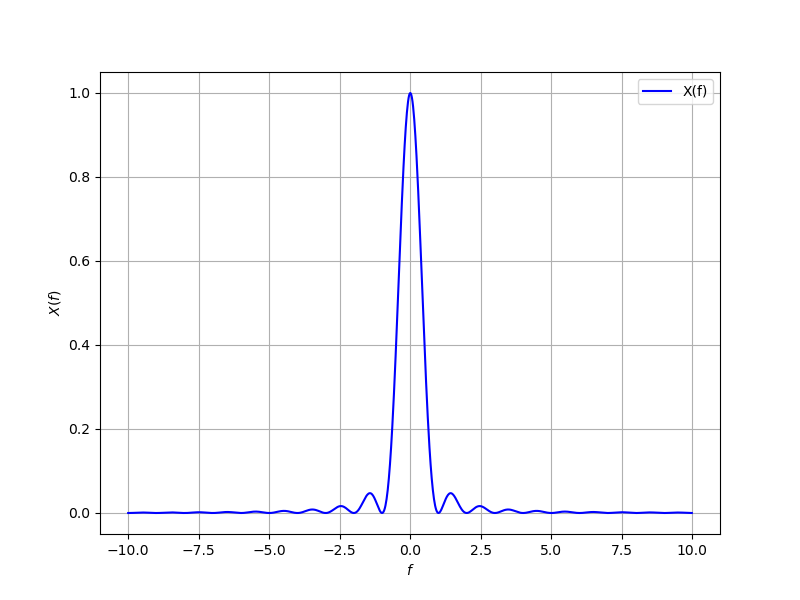
\includegraphics[width=1\linewidth]{2021/EE/43/figs/graph.png}
    \caption{plot of X(f)}
\end{figure}
%\end{document}

\pagebreak
\item Let $f(t)$ be an even function, i.e.$f(-t) = f(t)$ for all t.Let the Fourier transform of $f(t)$ be defined as $F(\omega) = \int_{-\infty}^{\infty} f(t) e^{-j \omega t} \, dt $ . Suppose $\dfrac{dF(\omega)}{d \omega} = -\omega F(\omega)$ for all $\omega$ , and $F(0) = 1$ . Then


\begin{enumerate}[label = (\Alph*)]
\item $f(0) < 1 $\\
\item  $f(0) > 1 $\\
\item  $f(0) = 1 $\\
\item   $f(0) = 0 $\\
\end{enumerate} \hfill{(GATE EE 2021)}\\
\solution
\iffalse
\let\negmedspace\undefined
\let\negthickspace\undefined
\documentclass[journal,12pt,twocolumn]{IEEEtran}
\usepackage{cite}
\usepackage{amsmath,amssymb,amsfonts,amsthm}
\usepackage{algorithmic}
\usepackage{graphicx}
\usepackage{textcomp}
\usepackage{xcolor}
\usepackage{txfonts}
\usepackage{listings}
\usepackage{enumitem}
\usepackage{mathtools}
\usepackage{gensymb}
\usepackage{comment}
\usepackage[breaklinks=true]{hyperref}
\usepackage{tkz-euclide} 
\usepackage{listings}
\usepackage{gvv}  
\usepackage{tikz}
\usepackage{circuitikz} 
\usepackage{caption}
\def\inputGnumericTable{}              
\usepackage[latin1]{inputenc}          
\usepackage{color}                    
\usepackage{array}                     
\usepackage{longtable}                 
\usepackage{calc}                     \usepackage{multirow}                  
\usepackage{hhline}                    
\usepackage{ifthen}                    
\usepackage{lscape}
\usepackage{amsmath}
\newtheorem{theorem}{Theorem}[section]
\newtheorem{problem}{Problem}
\newtheorem{proposition}{Proposition}[section]
\newtheorem{lemma}{Lemma}[section]
\newtheorem{corollary}[theorem]{Corollary}
\newtheorem{example}{Example}[section]
\newtheorem{definition}[problem]{Definition}
\newcommand{\BEQA}{\begin{eqnarray}}
\newcommand{\EEQA}{\end{eqnarray}}
\newcommand{\define}{\stackrel{\triangle}{=}}
\theoremstyle{remark}
\newtheorem{rem}{Remark}

%\bibliographystyle{ieeetr}
\begin{document}
%

\bibliographystyle{IEEEtran}




\title{
%	\logo{
G.A.T.E.

\large{EE1205 : Signals and Systems}

Indian Institute of Technology Hyderabad
%	}
}
\author{Chirag Garg

(EE23BTECH11206)
}	





\maketitle

\newpage



\bigskip

\renewcommand{\thefigure}{\theenumi}
\renewcommand{\thetable}{\theenumi}


\section{Question E.E.(32)}
\vspace{0.5cm}



\textbf{Question:} 
Let $f(t)$ be an even function, i.e.$f(-t) = f(t)$ for all t.Let the Fourier transform of $f(t)$ be defined as $F(\omega) = \int_{-\infty}^{\infty} f(t) e^{-j \omega t} \, dt $ . Suppose $\dfrac{dF(\omega)}{d \omega} = -\omega F(\omega)$ for all $\omega$ , and $F(0) = 1$ . Then


\begin{enumerate}[label = (\Alph*)]
\item $f(0) < 1 $\\
\item  $f(0) > 1 $\\
\item  $f(0) = 1 $\\
\item   $f(0) = 0 $\\
\end{enumerate} \hfill{(GATE EE 2021)}\\
%\section{Solution} 
\textbf{Solution: }
\fi
Given, \begin{align}
\dfrac{dF(\omega)}{d \omega} &= -\omega F(\omega) \\
\dfrac{dF(\omega)}{d \omega} + \omega F(\omega) &= 0 \\
ln|F(\omega)| &= -\dfrac{\omega^{2}}{2} + c \\
F(\omega) &= Ke^{-\frac{\omega^2}{2}}
\end{align}
Put $\omega = 0$ , \begin{align}
F(0) &= K \\
K&=1
\end{align}
\begin{align}
\therefore F(\omega) &= e^{-\frac{\omega^2}{2}}
\end{align}

\begin{center}
 $f(t) \longleftrightarrow F(\omega)$
\end{center}
 \begin{align}
e^{-at^{2}}  \longleftrightarrow  \sqrt{\dfrac{\pi}{a}}
e^{-\frac{\omega^2}{4a}} \; ; \; a > 0 \\
At \; a = \dfrac{1}{2} , \; e^{-\frac{t^{2}}{2}}  \longleftrightarrow  \sqrt{2\pi} e^{-\frac{\omega^2}{2}}\\
\dfrac{1}{\sqrt{2\pi}}e^{-\frac{t^{2}}{2}}  \longleftrightarrow  e^{-\frac{\omega^2}{2}} = F(\omega) \\
\text{Thus , } f(t) = \dfrac{1}{\sqrt{2\pi}}e^{-\frac{t^{2}}{2}} 
 \end{align}
 At $t = 0$  \begin{align}
 f(0) = \dfrac{1}{\sqrt{2\pi}} < 1
 \end{align}
 Hence , option (a) is correct.

\pagebreak
\item The exponential Fourier series representation of a continous-time periodic signal x\brak{t} is defined as\\
\begin{center}
$x\brak{t}=\sum\limits_{k=-\infty}^{\infty}a_ke^{jk\omega_0t}$\\
\end{center}
where $\omega_0$ is the fundamental angular frequency of x\brak{t} and the coefficients of the series are $a_k$.The following information is given about x\brak{t} and $a_k$\\
I. x\brak{t} is real and even,having a fundamental period of 6\\
II. The average value of x\brak{t} is 2.\\
III.\begin{align}
 a_k= \begin{cases} 
      k, & 1 \leq k \leq 3 \\
      0, &  k > 3 
   \end{cases}\\
   \end{align}
The average power of the signal x\brak{t} (rounded off to one decimal place) is \underline{\hspace{1cm}}. \\
\hfill(GATE EC 2021)\\
\solution\\
\iffalse
\let\negmedspace\undefined
\let\negthickspace\undefined
\documentclass[a4,12pt,onecolumn]{IEEEtran}
\usepackage{amsmath,amssymb,amsfonts,amsthm}
\usepackage{algorithmic}
\usepackage{graphicx}
\usepackage{textcomp}
\usepackage{xcolor}
\usepackage{txfonts}
\usepackage{listings}
\usepackage{enumitem}
\usepackage{mathtools}
\usepackage{gensymb}
\usepackage[breaklinks=true]{hyperref}
\usepackage{tkz-euclide}
\usepackage{listings}
\usepackage{circuitikz}
\usepackage{gvv}
\begin{document}
\title{
\Huge\textbf{ GATE 2021 Assignment}\\
\Huge\textbf{EE1205} Signals and Systems\\
}
\large\author{Kurre Vinay\\EE23BTECH11036}
\maketitle
\textbf{Question:}
The exponential Fourier series representation of a continous-time periodic signal x\brak{t} is defined as\\
\begin{center}
$x\brak{t}=\sum\limits_{k=-\infty}^{\infty}a_ke^{jk\omega_0t}$\\
\end{center}
where $\omega_0$ is the fundamental angular frequency of x\brak{t} and the coefficients of the series are $a_k$.The following information is given about x\brak{t} and $a_k$\\
I. x\brak{t} is real and even,having a fundamental period of 6\\
II. The average value of x\brak{t} is 2.\\
III.\begin{align}
 a_k= \begin{cases} 
      k, & 1 \leq k \leq 3 \\
      0, &  k > 3 
   \end{cases}\\
   \end{align}
The average power of the signal x\brak{t} (rounded off to one decimal place) is \underline{\hspace{1cm}}. \\
\hfill(GATE EC 2021)\\
\solution\\
\fi
\begin{table}[ht!]
\begin{center}
\begin{tabular}{|c|c|c|}
   \hline
   variable&value&description\\
   \hline
   $T_0$&6&Fundamental time period\\
   \hline
  $P_{avg}$&-&average power of the signal\\
   \hline
   x\brak{t}&$\sum\limits_{k=-\infty}^{\infty}a_ke^{jk\omega_0t}$&Input signal\\
   \hline
   $a_k$& $\begin{cases} 
      k, & 1 \leq k \leq 3 \\
      0, &  k > 3 
   \end{cases}$&coefficients of the series \\
   \hline
  $a_0$&2&average of x\brak{t}\\
   \hline
\end{tabular}
\caption{Table: Input Parameters}
\end{center}
\end{table}\\
x\brak{t} is even and real so, $a_k$=$a_{-k}$\\
Parswal's Power Theorem\\
Proof
\begin{align}
P&=\frac{1}{T}\int\limits_{\frac{-T}{2}}^{\frac{T}{2}}\left| x\brak{t}^2 \right|dt ,\quad{\left| x\brak{t}^2 \right|=x\brak{t}x^*\brak{t}}\\
P&=\frac{1}{T}\int\limits_{\frac{-T}{2}}^{\frac{T}{2}}x\brak{t}x^*\brak{t}dt \\
x\brak{t}&=\sum\limits_{n=-\infty}^{\infty}C_ne^{jn\omega_0t}\\
P&=\frac{1}{T}\int\limits_{\frac{-T}{2}}^{\frac{T}{2}}\brak{\sum\limits_{k=-\infty}^{\infty}C_ne^{jn\omega_0t}}x^*\brak{t}dt\\
P&=\sum\limits_{n=-\infty}^{\infty}C_n\brak{\frac{1}{T}\int\limits_{\frac{-T}{2}}^{\frac{T}{2}}x^*\brak{t}e^{jn\omega_0t}dt}\\
&=\sum\limits_{n=-\infty}^{\infty}C_nC^*_n\\
\implies P&=\sum\limits_{n=-\infty}^{\infty}\left| C_n \right|^2
\end{align}
By using Parsval's Power Theorem
\begin{align}
\frac{1}{T}\int\limits_{0}^{T}\left| x\brak{t}^2 \right|dt&=\sum\limits_{k=-\infty}^{\infty}\left| a_k \right|^2\\
P_{avg}&=\sum\limits_{k=-\infty}^{\infty}\left| a_k \right|^2\\
&=2\sum\limits_{k=1}^{\infty}\left| a_k \right|^2 +|a_0|^2\\
&=2\sum\limits_{k=1}^{3}\left| a_k \right|^2  +|a_0|^2 \\
&=2\brak{1^2+2^2+3^2}+2^2\\
&=32\\
x\brak{n}&=2\text{Re}\brak{e^{\frac{j\pi t}{3}}+2e^{\frac{2j\pi t}{3}}+3e^{j\pi t}} + 2\\
\implies x\brak{n}&=2\brak{cos\brak{\frac{\pi t}{3}}+2cos\brak{\frac{2\pi t}{3}}+3cos\brak{\pi t}} + 2
\end{align}
The average power of the signal x\brak{t} (rounded off to one decimal place) is $32$
\begin{figure}[ht!]
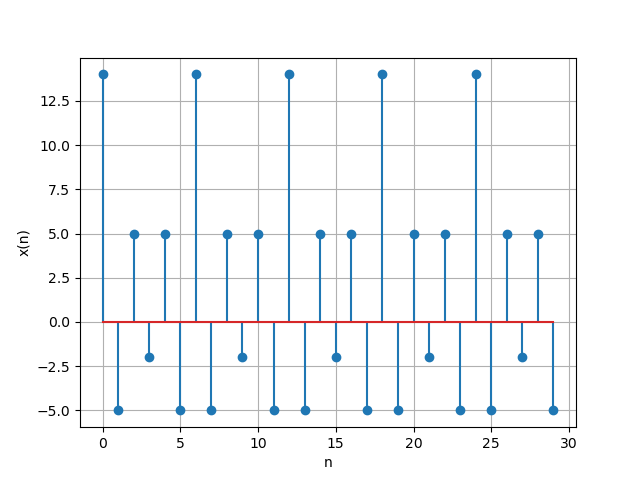
\includegraphics[width=\columnwidth]{2021/EC/39/figs/fig.png}
\caption{\large{STEM PLOT OF $y\brak{n}$}}
\end{figure}


\pagebreak

\end{enumerate}
